\clearpage
\setcounter{page}{1}
\maketitlesupplementary

\setcounter{section}{0}
\renewcommand{\thesection}{\Alph{section}}
\renewcommand{\theHsection}{supp.\arabic{section}}
\setcounter{table}{0}
\renewcommand{\thetable}{S\arabic{table}}
\renewcommand{\theHtable}{supp.\arabic{table}}
\setcounter{figure}{0}
\renewcommand{\thefigure}{S\arabic{figure}}
\renewcommand{\theHfigure}{supp.\arabic{figure}}

% Compiled only when main.tex sets \suppltrue.
% Sections here can be referenced from the main paper (e.g. \cref{sec:supp_impl}) and vice versa.

% ---- 可能的内容（写完删除）--------------------------------------------------
% 实现细节与超参数；统计协议（配对方式、McNemar、CI）；逐任务完整结果；
% 额外的分析与可视化；运行时间测量方式；失败案例；视频说明。
% ---------------------------------------------------------------------------

\section{Implementation Details}
\label{sec:supp_impl}

The main text specifies the LIBERO training and evaluation settings.
The Object router uses pure distillation during router training, while all budget-specific decoder adapters use distillation plus the 0.02-weight ground-truth term.
Bridge uses its separately trained pure-distillation router; its training data and camera setup differ from LIBERO.
For DiT4DiT, the 442-token LIBERO setting pools all future spatial groups and additionally coarsens the observed slice; it is not the 589-token future allocation with only the observation budget changed.

\section{Statistical and Efficiency Details}
\label{sec:supp_stats}

% Paired comparisons of ARROW on mimic-video: against native (left) and against the full-context LoRA control (right).
% 2026-11-11: the two former tables (ours vs native; mimic-video rows of ours vs native + LoRA) were merged here.
% The DiT4DiT differences of the former second table are given in the text of the supplement.
\begin{table*}[t]
  \centering
  \caption{\textbf{Paired comparisons of \method on mimic-video.}
  Every cell has 500 paired episodes.
  $\Delta$ is \method minus the reference in percentage points, with unadjusted paired Wald 95\% intervals.
  $p_H$ is Holm-corrected; each reference forms its own family of nine tests.
  The nominal Object 30\% intervals do not establish significance after correction.}
  \label{tab:paired_uncertainty}
  \small
  \setlength{\tabcolsep}{6pt}
  \begin{tabular}{lr lr lr}
    \toprule
    & & \multicolumn{2}{c}{vs.\ native} & \multicolumn{2}{c}{vs.\ native + LoRA} \\
    \cmidrule(lr){3-4} \cmidrule(lr){5-6}
    Suite & Future & $\Delta$ [95\% CI] & $p_H$ & $\Delta$ [95\% CI] & $p_H$ \\
    \midrule
    Spatial & 10\% & $-19.6$ [$-24.0$, $-15.2$] & $4.8\!\times\!10^{-16}$ & $-20.8$ [$-25.0$, $-16.6$] & $1.4\!\times\!10^{-19}$ \\
    Spatial & 20\% & $-2.2$ [$-5.4$, $+1.0$] & 1.00 & $-3.4$ [$-6.4$, $-0.4$] & 0.24 \\
    Spatial & 30\% & $+1.6$ [$-1.2$, $+4.4$] & 1.00 & $+0.4$ [$-2.4$, $+3.2$] & 1.00 \\
    \addlinespace[2pt]
    Object & 10\% & $-0.2$ [$-2.8$, $+2.4$] & 1.00 & $+0.6$ [$-2.1$, $+3.3$] & 1.00 \\
    Object & 20\% & $+0.0$ [$-2.3$, $+2.3$] & 1.00 & $+0.8$ [$-1.6$, $+3.2$] & 1.00 \\
    Object & 30\% & $+2.4$ [$+0.3$, $+4.5$] & 0.25 & $+3.2$ [$+0.9$, $+5.5$] & 0.063 \\
    \addlinespace[2pt]
    Goal & 10\% & $-15.4$ [$-19.6$, $-11.2$] & $1.6\!\times\!10^{-11}$ & $-15.0$ [$-19.3$, $-10.7$] & $2.2\!\times\!10^{-10}$ \\
    Goal & 20\% & $-0.8$ [$-4.0$, $+2.4$] & 1.00 & $-0.4$ [$-3.6$, $+2.8$] & 1.00 \\
    Goal & 30\% & $+0.0$ [$-2.9$, $+2.9$] & 1.00 & $+0.4$ [$-2.5$, $+3.3$] & 1.00 \\
    \bottomrule
  \end{tabular}
\end{table*}


Confidence intervals describe paired episode differences, not variation over independently trained models.
All adapter configurations use one training seed.
The nine mimic-video ours--native comparisons in the main table use a common Holm family; its Object 30\% adjusted $p$-value is 0.250.
The deletion reference comparisons are separate from that family and do not change the dagger marks.
The original Goal/Object ours--deletion analysis uses a post-hoc family of 12 contrasts, as documented with the results.

The timing benchmark uses Spatial checkpoints on an exclusively allocated H100, batch size one, with text encoding included.
There are three warmup calls and eight interleaved rounds of four calls per arm; reported values are medians of 32 synchronized wall-clock measurements.
The graphed native reference is 701.7\,ms; the eager native reference has median 770.4\,ms across the three budget runs.
The deployed 10\%/20\%/30\% configurations run in 404.2/440.7/477.1\,ms and use 35.7/42.7/49.6 TFLOPs per query.
Speedups relative to graphed native are reported in the main text; relative to the pooled eager reference they are approximately $1.91\times$, $1.75\times$ and $1.61\times$.
The folded-adapter configuration is the one used for timing; these measurements are not a separate closed-loop evaluation of graph/fold equivalence.
For DiT4DiT, an exclusively allocated H100 runs ten warmup calls and 50 measured calls per configuration, with batch size one and no CUDA graphs.
The synchronized wall-clock measurement includes the single-frame VAE and uses cached text; native and compressed configurations share both conventions and stop at the action head's extraction layer.
Native takes 57.7\,ms; the evaluated 589/442/391-token configurations with unfused LoRA take 66.2/66.6/66.9\,ms.
Separate stage measurements show backbone time of 21.7\,ms for native versus 24.2--24.5\,ms compressed, and action-head time of 22.1\,ms versus 28.6--28.7\,ms with LoRA.
These measurements establish overhead at these stages, but do not isolate a kernel-level cause.
Disabling the LoRA branch gives a 60.2--60.9\,ms compute proxy; a policy with folded trained weights has not been validated, so this proxy is not substituted for the evaluated latency.

The earlier DiT4DiT FLOPs comparison uses a released 4.91-TFLOP pipeline with a padded VAE encode.
Encoding only the real observed frame reduces this to 2.90 TFLOPs and is shared by native and ours.
With this common change, the evaluated 589/442/391-token configurations use 2.45/2.10/1.98 TFLOPs including VAE; the main table excludes the common 0.67-TFLOP VAE cost.
Thus the earlier reductions relative to the released path describe arithmetic, not wall-clock speedup or compression alone.
\TODO{Numerical equivalence checks for the deployed mimic-video fold/graph configuration and deletion/external-method timing.}

\section{Original External-Policy Adaptations}
\label{sec:supp_original_external}

% Source: main_results_dit4dit_sources.json; original 2026-11-05 protocol.
\begin{table*}[t]
  \centering
  \caption{\textbf{Original external-policy adaptations on DiT4DiT.}
  These results retain the initial observation-preserving selectors, VLA-Pruner's three dense warm-start queries and ADP's trajectory-gated dense fallback.
  Target is the compressed-branch length; Mean is the per-episode mean context averaged across all three suites, including dense calls.
  Each completed success rate uses 500 paired episodes.
  CF-sel.'s additional full-context probe is extra work beyond the retained context; no-LoRA is the training-free selection arm.
  These are distinct from the fixed-budget selection ports described in this section.}
  \label{tab:dit4dit_original_external}
  \footnotesize
  \setlength{\tabcolsep}{5pt}
  \begin{tabular}{lrrrrrr}
    \toprule
    Original adaptation & Target & Mean context & Spatial & Object & Goal & Avg. \\
    \midrule
    FastV-style & 589 & 589.0 & 98.0 & 100.0 & 98.4 & 98.8 \\
    VLA-Pruner & 589 & 630.9 & 98.6 & 99.6 & 98.8 & 99.0 \\
    ADP & 589 & 703.4 & 98.0 & 99.8 & 97.6 & 98.5 \\
    CF-sel. + LoRA & 589 & \TODO{--} & 98.8 & \TODO{--} & 98.6 & \TODO{--} \\
    CF-sel., no LoRA & 589 & 589.0 & 98.4 & 100.0 & 98.4 & 98.9 \\
    \midrule
    FastV-style & 442 & 442.0 & 94.4 & 99.4 & 92.4 & 95.4 \\
    VLA-Pruner & 442 & \TODO{--} & 97.4 & \TODO{--} & 97.8 & \TODO{--} \\
    ADP & 442 & 638.5 & 98.4 & 99.6 & 98.4 & 98.8 \\
    CF-sel. + LoRA & 442 & 442.0 & 97.2 & 99.2 & 96.4 & 97.6 \\
    CF-sel., no LoRA & 442 & 442.0 & 96.2 & 97.8 & 93.6 & 95.9 \\
    \bottomrule
  \end{tabular}
\end{table*}


The original VLA-Pruner and ADP adaptations use more context than their compressed-branch targets because of dense calls (\cref{tab:dit4dit_original_external}).
They therefore do not constitute fixed-context comparisons.
The main table instead reserves explicit fixed-budget selection ports (FB), with 392/197, 344/98 and 293/98 observed/future tokens at 589, 442 and 391 total context tokens.
ADP-sel. removes trajectory-gated dense fallback and tests the text-guided selection component.
VLA-sel. uses three semantic-only compressed bootstrap queries and scatters their action attention to source positions before maintaining its causal history.
FastV-style and CF-sel. also select observation tokens at the two lower budgets; their selection scores and source positions remain method-specific.
CF-sel. retains a paid full-context probe, which must be included in its inference cost.
All fixed-context ports use a fresh matched decoder adapter; their old-policy success rates are not reused.

\section{Additional Transfer and Router-Training Results}
\label{sec:supp_transfer}

With 100 full-resolution groups, the three Bridge budgets give 20/96, 24/96 and 27/96 successes, versus 46/96 for native.
Their paired differences are $-27.1$ [$-38.1$,$-16.1$], $-22.9$ [$-32.7$,$-13.1$] and $-19.8$ [$-29.6$,$-9.9$] percentage points, with exact McNemar $p=1.3\times10^{-5}$, $2.7\times10^{-5}$ and $3.1\times10^{-4}$, respectively.
These failed points motivate reporting the entire higher-budget $F=200$ sweep rather than only its best point estimate.

The original $F=200$, 11,400-token run gives 45/96 successes (46.9\%), versus 46/96 for native; its paired difference is $-1.0$ points [95\% CI $-9.9$,$+7.9$], with discordant counts 9/10 and exact McNemar $p=1.00$.
The 50.0\% point estimate in the transfer table comes from a separate run on another machine with a different seed.
Its interval and paired comparison remain pending; the original run's interval is not reused for it.

Earlier combined spatial/temporal DiT4DiT configurations on GR1 have lower point estimates than native.
For example, the future-space/time 441-token configuration with 41 full-resolution groups reaches 53.2\%, versus 54.9\% for native, a $-1.8$ point difference with interval [$-4.5$,$+1.0$].
The completed 466-token follow-up keeps 41 future $2\times2$ groups at full resolution and merges 74 spatial tubes across time; it removes 48 tokens spatially and 74 temporally while leaving the observation unchanged.
Its frozen router and 1,500-step decoder adapter yield 660/1,200 successes, versus 659/1,200 for native.
The paired difference is $+0.08$ points [95\% CI $-2.66$,$+2.83$], with discordant counts 142/141 and exact McNemar $p=1.00$.
This configuration was selected after inspecting the intermediate 441-token results and uses one training seed.
It demonstrates simultaneous spatial and temporal allocation in this evaluated setting, but its confidence interval does not establish equivalence to native.

Continuing to train the router jointly with the adapter for 1,500 steps gives the following success rates, in 10\%/20\%/30\% budget order:
Spatial 72.2/90.8/91.6\%, Goal 76.2/86.2/89.4\%, and Object 91.8/94.4/96.0\%.
Relative to frozen-router training, no improvement survives Holm correction over nine suite--budget comparisons; the pooled, post-hoc paired test has $p=0.83$.
The individual adjusted $p$-values, in the same order, are 1.00/0.68/1.00, 1.00/0.10/1.00 and 0.77/1.00/1.00.
This is a lack of detected benefit for that recipe and sample size, not evidence of equivalence.

\section{Detailed Action-Relevance Analysis}
\label{sec:supp_relevance}

\begin{figure*}[t]
  \centering
  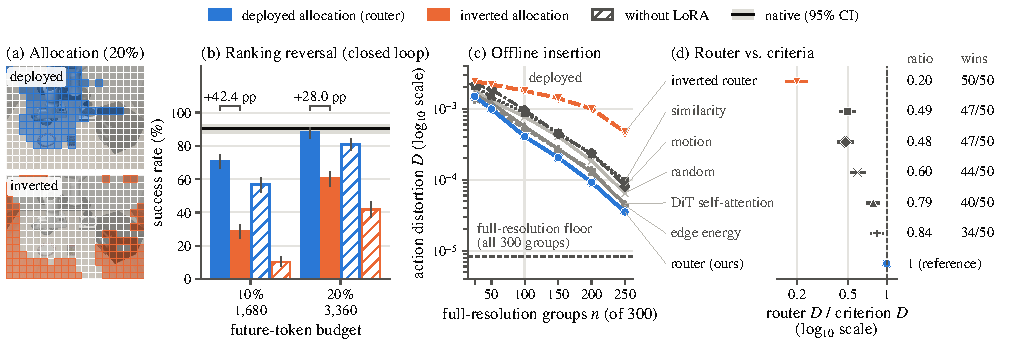
\includegraphics[width=\linewidth]{fig5_action_relevance.pdf}
  \caption{\textbf{Ranking reversal and offline action distortion.}
  (a) Deployed and inverted full-resolution groups at the same budget.
  (b) Spatial success over 500 paired episodes, with separately trained low-rank adapters (solid) or without adapters (hatched); bars show Wilson 95\% confidence intervals.
  (c) Spatial insertion curves over 200 windows from 50 held-out episodes: the top-$n$ groups retain full resolution, the rest are merged, and all 14 future frames remain.
  Distortion is the normalized mean squared difference from the native decoder's first five actions under full context, geometrically averaged over windows.
  The dashed line is the full-resolution numerical floor.
  (d) Router-to-criterion distortion ratios, averaged over six group counts in log space, with episode-level Student's $t$ 95\% intervals.
  The five criteria are similarity, motion, block-2 self-attention, observed-frame edge energy and random selection.}
  \label{fig:supp_relevance}
\end{figure*}

The pre-registered offline family also included full-context decoder cross-attention, which has approximately 7\% lower distortion than the router ($p=0.0078$ after correction).
It requires completing the uncompressed video/decoder forward pass and therefore is not an equal-cost block-2 scoring substitute.
Claims of superiority apply only to the five task-agnostic criteria shown in the figure.
Similarity ranking in this analysis is not a complete ToMe implementation.
The matched offline coverage-versus-resolution comparison does not distinguish the two allocations after correction, so it is not used to attribute the closed-loop operator gap to coarse coverage alone.

\section{Absolute Cross-Policy Success Rates}
\label{sec:supp_absolute}

\begin{table*}[t]
  \centering
  \caption{\textbf{Absolute LIBERO success rates for context.}
  Avg. is recomputed over Spatial/Object/Goal only; LIBERO-Long is omitted for every row.
  Published rows have different training, sensing and evaluation protocols and are not matched compression baselines.
  Source links identify the actual result table or release, including secondary reporting where used.
  Our rows repeat \mainref{tab:main_results}{Table~1}.
  The table also includes SmolVLA and Cosmos Policy, which are omitted from the parameter bubble figure.}
  \label{tab:absolute_success}
  \small
  \setlength{\tabcolsep}{6pt}
  \begin{tabular}{lrrrrl}
    \toprule
    Policy & Spatial & Object & Goal & Avg. & Result source \\
    \midrule
    OpenVLA & 84.7 & 88.4 & 79.2 & 84.1 & \href{https://arxiv.org/abs/2406.09246}{App. E} \\
    OpenVLA-OFT & 97.6 & 98.4 & 97.9 & 98.0 & \href{https://arxiv.org/abs/2502.19645}{Tab. I} \\
    $\pi_0$ & 96.8 & 98.8 & 95.8 & 97.1 & \href{https://arxiv.org/abs/2502.19645}{Tab. I} \\
    $\pi_{0.5}$ & 98.8 & 98.2 & 98.0 & 98.3 & \href{https://huggingface.co/docs/lerobot/libero}{OpenPI results} \\
    $\pi_0$-FAST & 96.4 & 96.8 & 88.6 & 93.9 & \href{https://arxiv.org/abs/2502.19645}{Tab. I} \\
    Octo & 78.9 & 85.7 & 84.6 & 83.1 & \href{https://arxiv.org/abs/2406.09246}{App. E} \\
    SpatialVLA & 88.2 & 89.9 & 78.6 & 85.6 & \href{https://arxiv.org/abs/2501.15830}{Tab. III} \\
    CoT-VLA & 87.5 & 91.6 & 87.6 & 88.9 & \href{https://arxiv.org/abs/2503.22020}{LIBERO results} \\
    UniVLA & 96.5 & 96.8 & 95.6 & 96.3 & \href{https://arxiv.org/abs/2505.06111}{Tab. I} \\
    NORA-Long & 92.2 & 95.4 & 89.4 & 92.3 & \href{https://arxiv.org/abs/2504.19854}{Tab. 2} \\
    VLA-RL & 90.2 & 91.8 & 82.2 & 88.1 & \href{https://arxiv.org/abs/2505.18719}{Tab. 1} \\
    WorldVLA & 87.6 & 96.2 & 83.4 & 89.1 & \href{https://arxiv.org/abs/2506.21539}{Tab. 2} \\
    SmolVLA (0.45B) & 90.0 & 96.0 & 92.0 & 92.7 & \href{https://arxiv.org/html/2506.01844v1}{Tab. 2} \\
    SmolVLA (2.25B) & 93.0 & 94.0 & 91.0 & 92.7 & \href{https://arxiv.org/html/2506.01844v1}{Tab. 2} \\
    Cosmos Policy & 98.1 & 100.0 & 98.2 & 98.8 & \href{https://research.nvidia.com/labs/cosmos-lab/cosmos-policy/}{Author results} \\
    \midrule
    mimic-video native & 90.4 & 94.0 & 90.2 & 91.5 & Our evaluation \\
    mimic-video+ (20\% future) & 88.2 & 94.0 & 89.4 & 90.5 & Our evaluation \\
    DiT4DiT native & 98.6 & 99.4 & 98.6 & 98.9 & Our evaluation \\
    DiT4DiT+ (589 tokens) & 99.2 & 100.0 & 98.6 & 99.3 & Our evaluation \\
    \bottomrule
  \end{tabular}
\end{table*}


The results in \cref{tab:absolute_success} provide context rather than a common-backbone or common-protocol comparison.
The main claims concern changes relative to each policy's own native backbone.
For $\pi_0$ and $\pi_0$-FAST, the listed numbers are the released-model results tabulated by OpenVLA-OFT; $\pi_{0.5}$ uses the OpenPI release numbers reproduced in the LeRobot documentation.
The three-suite means are recomputed, rather than copied from four-suite LIBERO averages.

\begin{figure*}[t]
  \centering
  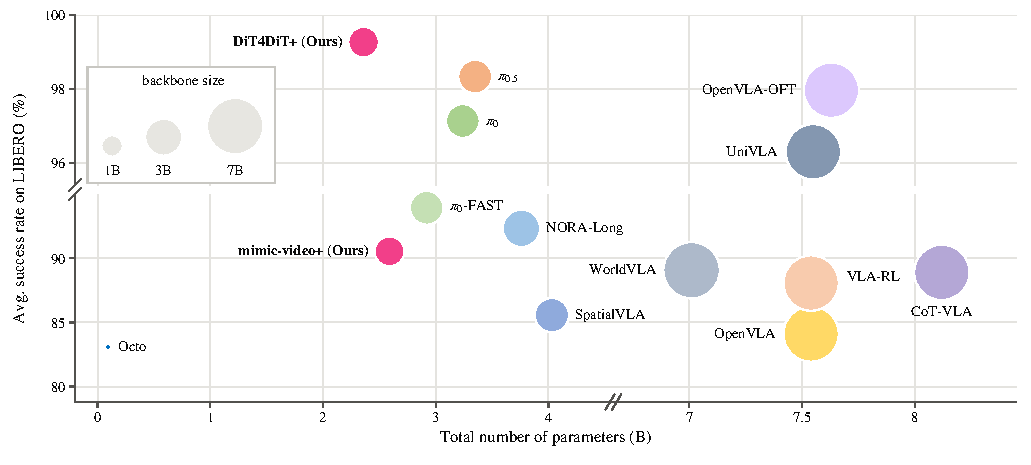
\includegraphics[width=\linewidth]{fig_bubble_params.pdf}
  \caption{\textbf{Performance versus model size on LIBERO.}
  Points show three-suite mean success; the horizontal axis is total parameter count and circle area represents backbone size.
  Our points use 20\% of mimic-video's future tokens and 589/784 DiT4DiT tokens.
  The plot uses a selected set of policies and omits frozen instruction encoders from parameter totals; the table above includes the omitted SmolVLA and Cosmos Policy results and both native evaluations.
  This figure does not establish a matched efficiency comparison across architectures.}
  \label{fig:supp_bubble}
\end{figure*}
